\documentclass[border=8pt]{standalone}
\usepackage{fontspec}
\setmainfont{TeX Gyre Heros}[Ligatures=TeXOff]
\XeTeXgenerateactualtext=1
\setsansfont{TeX Gyre Heros}
\usepackage{tikz}
\usetikzlibrary{arrows.meta,positioning,shapes.geometric,shapes.misc,shapes.symbols,fit,backgrounds,calc,chains}
\definecolor{ink}{HTML}{111827}
\definecolor{band}{HTML}{F3F4F6}
\definecolor{band2}{HTML}{E5E7EB}
\definecolor{accent}{HTML}{1D4ED8}
\definecolor{accentlight}{HTML}{DBEAFE}
\definecolor{warn}{HTML}{B91C1C}
\definecolor{warnlight}{HTML}{FEE2E2}
\definecolor{ok}{HTML}{047857}
\definecolor{oklight}{HTML}{D1FAE5}
\tikzset{
  >={Stealth[length=2.6mm]},
  box/.style={draw=ink, line width=0.6pt, rounded corners=9pt, fill=white, align=center,
              inner sep=4pt, font=\small},
  pill/.style={box, rounded corners=13pt},
  key/.style={box, fill=accentlight, draw=accent, line width=0.9pt},
  soft/.style={box, fill=band},
  dec/.style={draw=ink, line width=0.6pt, diamond, aspect=2.2, align=center, inner sep=1.5pt,
              font=\footnotesize, fill=white},
  arr/.style={->, draw=ink, line width=0.6pt},
  darr/.style={->, draw=ink, line width=0.6pt, dashed},
  lbl/.style={font=\footnotesize, fill=white, inner sep=1.5pt},
  layer/.style={draw=band2, fill=band, rounded corners=6pt},
  title/.style={font=\bfseries\small, align=left, anchor=west},
}
\begin{document}
\sffamily\hyphenpenalty=10000\exhyphenpenalty=10000

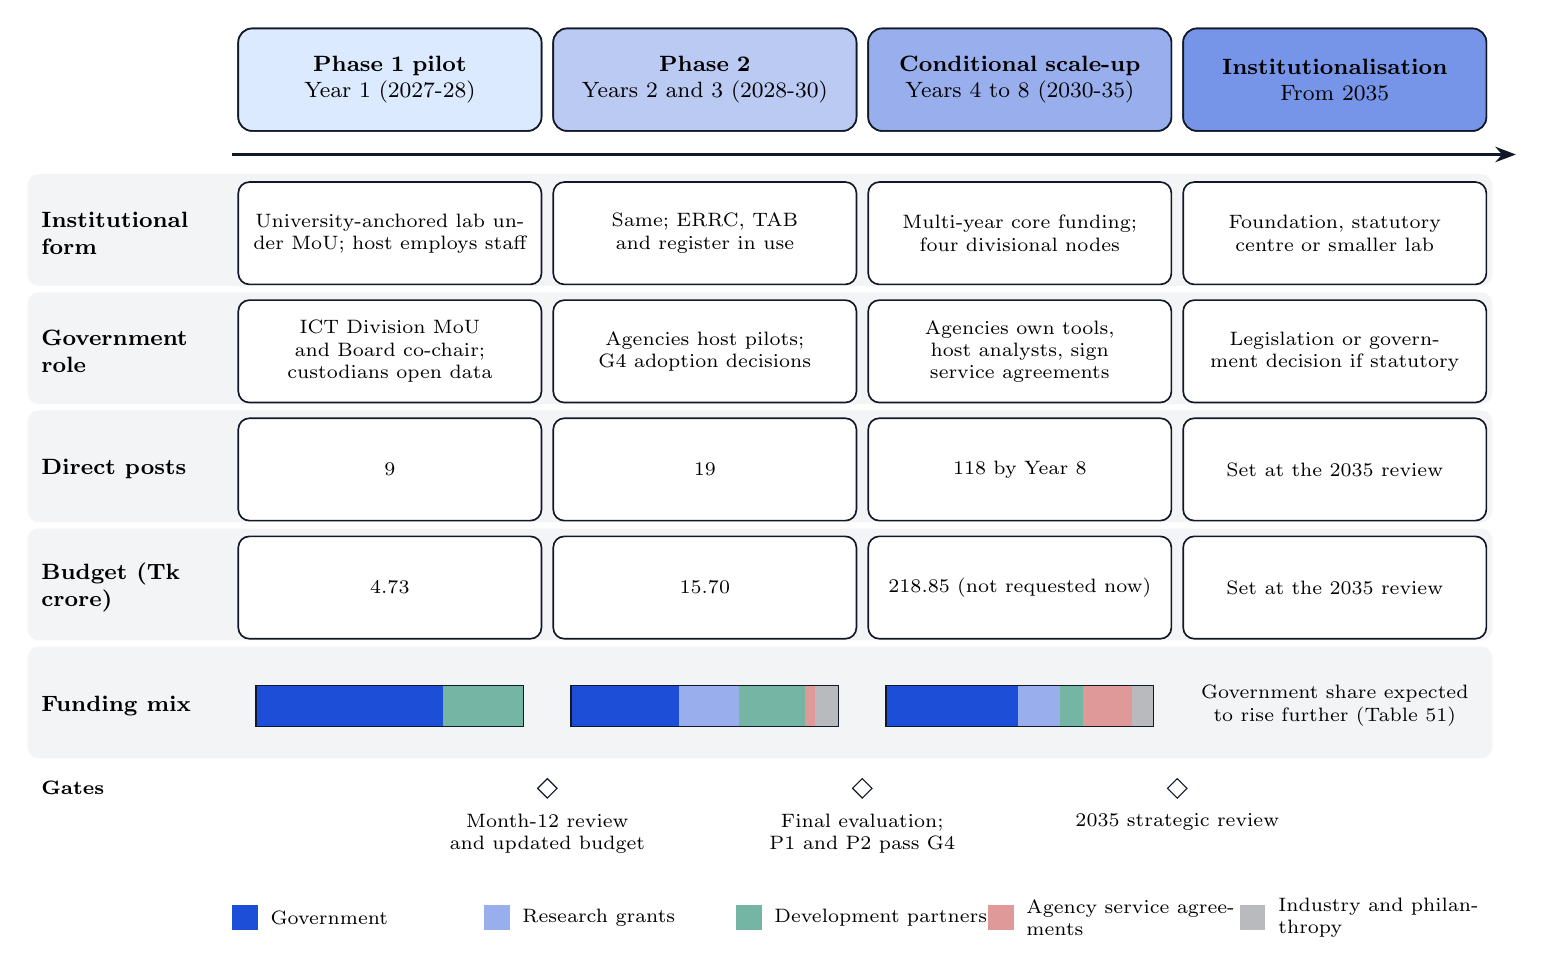
\begin{tikzpicture}
\def\L{26mm}\def\C{40mm}\def\R{15mm}
\tikzset{hd/.style={box, rounded corners=5pt, minimum width=\C-1.5mm, minimum height=13mm, text width=\C-3mm, font=\footnotesize, inner sep=2pt},
         cell/.style={box, rounded corners=4pt, minimum width=\C-1.5mm, minimum height=\R-2mm, text width=\C-4mm, font=\scriptsize, inner sep=1.5pt},
         ln/.style={font=\footnotesize\bfseries, text width=\L-3mm, align=left, anchor=west}}
\foreach \c/\col in {0/accentlight,1/accent!30,2/accent!45,3/accent!60} {
  \node[hd, fill=\col] (h\c) at (\L+\c*\C+0.5*\C, 0) {};
}
\node[hd, fill=accentlight] at (h0) {\textbf{Phase 1 pilot}\\Year 1 (2027-28)}; \node[hd, fill=accent!30] at (h1) {\textbf{Phase 2}\\Years 2 and 3 (2028-30)};
\node[hd, fill=accent!45] at (h2) {\textbf{Conditional scale-up}\\Years 4 to 8 (2030-35)}; \node[hd, fill=accent!60] at (h3) {\textbf{Institutionalisation}\\From 2035};
\draw[arr, line width=1.2pt] (\L,-9.5mm) -- (\L+4*\C+3mm,-9.5mm);
\newcommand{\lane}[6]{%
  \fill[band, rounded corners=4pt] (0,-12mm-#1*\R) rectangle (\L+4*\C,-12mm-#1*\R-\R+0.8mm);
  \node[ln] at (0.5mm,-12mm-#1*\R-0.5*\R) {#2};
  \node[cell] at (\L+0.5*\C,-12mm-#1*\R-0.5*\R) {#3};
  \node[cell] at (\L+1.5*\C,-12mm-#1*\R-0.5*\R) {#4};
  \node[cell] at (\L+2.5*\C,-12mm-#1*\R-0.5*\R) {#5};
  \node[cell] at (\L+3.5*\C,-12mm-#1*\R-0.5*\R) {#6};}
\lane{0}{Institutional form}{University-anchored lab under MoU; host employs staff}{Same; ERRC, TAB and register in use}{Multi-year core funding; four divisional nodes}{Foundation, statutory centre or smaller lab}
\lane{1}{Government role}{ICT Division MoU and Board co-chair; custodians open data}{Agencies host pilots; G4 adoption decisions}{Agencies own tools, host analysts, sign service agreements}{Legislation or government decision if statutory}
\lane{2}{Direct posts}{9}{19}{118 by Year 8}{Set at the 2035 review}
\lane{3}{Budget (Tk crore)}{4.73}{15.70}{218.85 (not requested now)}{Set at the 2035 review}
\fill[band, rounded corners=4pt] (0,-12mm-4*\R) rectangle (\L+4*\C,-12mm-4*\R-\R+0.8mm);
\node[ln] at (0.5mm,-12mm-4*\R-0.5*\R) {Funding mix};
\fill[accent] ($(\L+0*\C+3mm+0.0000*\C-0.0000*6mm, -12mm-4*\R-0.5*\R-2.6mm)$) rectangle ($(\L+0*\C+3mm+0.7000*\C-0.7000*6mm, -12mm-4*\R-0.5*\R+2.6mm)$);
\fill[ok!55] ($(\L+0*\C+3mm+0.7000*\C-0.7000*6mm, -12mm-4*\R-0.5*\R-2.6mm)$) rectangle ($(\L+0*\C+3mm+1.0000*\C-1.0000*6mm, -12mm-4*\R-0.5*\R+2.6mm)$);
\draw[ink, line width=0.4pt] (\L+0*\C+3mm, -12mm-4*\R-0.5*\R-2.6mm) rectangle (\L+0*\C+\C-3mm, -12mm-4*\R-0.5*\R+2.6mm);
\fill[accent] ($(\L+1*\C+3mm+0.0000*\C-0.0000*6mm, -12mm-4*\R-0.5*\R-2.6mm)$) rectangle ($(\L+1*\C+3mm+0.4023*\C-0.4023*6mm, -12mm-4*\R-0.5*\R+2.6mm)$);
\fill[accent!45] ($(\L+1*\C+3mm+0.4023*\C-0.4023*6mm, -12mm-4*\R-0.5*\R-2.6mm)$) rectangle ($(\L+1*\C+3mm+0.6262*\C-0.6262*6mm, -12mm-4*\R-0.5*\R+2.6mm)$);
\fill[ok!55] ($(\L+1*\C+3mm+0.6262*\C-0.6262*6mm, -12mm-4*\R-0.5*\R-2.6mm)$) rectangle ($(\L+1*\C+3mm+0.8738*\C-0.8738*6mm, -12mm-4*\R-0.5*\R+2.6mm)$);
\fill[warn!45] ($(\L+1*\C+3mm+0.8738*\C-0.8738*6mm, -12mm-4*\R-0.5*\R-2.6mm)$) rectangle ($(\L+1*\C+3mm+0.9105*\C-0.9105*6mm, -12mm-4*\R-0.5*\R+2.6mm)$);
\fill[ink!30] ($(\L+1*\C+3mm+0.9105*\C-0.9105*6mm, -12mm-4*\R-0.5*\R-2.6mm)$) rectangle ($(\L+1*\C+3mm+1.0000*\C-1.0000*6mm, -12mm-4*\R-0.5*\R+2.6mm)$);
\draw[ink, line width=0.4pt] (\L+1*\C+3mm, -12mm-4*\R-0.5*\R-2.6mm) rectangle (\L+1*\C+\C-3mm, -12mm-4*\R-0.5*\R+2.6mm);
\fill[accent] ($(\L+2*\C+3mm+0.0000*\C-0.0000*6mm, -12mm-4*\R-0.5*\R-2.6mm)$) rectangle ($(\L+2*\C+3mm+0.4942*\C-0.4942*6mm, -12mm-4*\R-0.5*\R+2.6mm)$);
\fill[accent!45] ($(\L+2*\C+3mm+0.4942*\C-0.4942*6mm, -12mm-4*\R-0.5*\R-2.6mm)$) rectangle ($(\L+2*\C+3mm+0.6500*\C-0.6500*6mm, -12mm-4*\R-0.5*\R+2.6mm)$);
\fill[ok!55] ($(\L+2*\C+3mm+0.6500*\C-0.6500*6mm, -12mm-4*\R-0.5*\R-2.6mm)$) rectangle ($(\L+2*\C+3mm+0.7351*\C-0.7351*6mm, -12mm-4*\R-0.5*\R+2.6mm)$);
\fill[warn!45] ($(\L+2*\C+3mm+0.7351*\C-0.7351*6mm, -12mm-4*\R-0.5*\R-2.6mm)$) rectangle ($(\L+2*\C+3mm+0.9200*\C-0.9200*6mm, -12mm-4*\R-0.5*\R+2.6mm)$);
\fill[ink!30] ($(\L+2*\C+3mm+0.9200*\C-0.9200*6mm, -12mm-4*\R-0.5*\R-2.6mm)$) rectangle ($(\L+2*\C+3mm+1.0000*\C-1.0000*6mm, -12mm-4*\R-0.5*\R+2.6mm)$);
\draw[ink, line width=0.4pt] (\L+2*\C+3mm, -12mm-4*\R-0.5*\R-2.6mm) rectangle (\L+2*\C+\C-3mm, -12mm-4*\R-0.5*\R+2.6mm);
\node[cell, draw=none, fill=none] at (\L+3.5*\C,-12mm-4*\R-0.5*\R) {Government share expected to rise further (Table 51)};
\foreach \c/\t in {1/{Month-12 review and updated budget},2/{Final evaluation; P1 and P2 pass G4},3/{2035 strategic review}} {
  \node[draw=ink, fill=white, diamond, inner sep=1.8pt] at (\L+\c*\C,-12mm-5*\R-3mm) {};
  \node[font=\scriptsize, anchor=north, text width=\C-6mm, align=center] at (\L+\c*\C,-12mm-5*\R-5mm) {\t};
}
\node[font=\scriptsize\bfseries, anchor=west] at (0.5mm,-12mm-5*\R-3mm) {Gates};
\foreach \i/\col/\t in {0/accent/{Government},1/accent!45/{Research grants},2/ok!55/{Development partners},3/warn!45/{Agency service agreements},4/ink!30/{Industry and philanthropy}} {
  \fill[\col] (\L+\i*0.8*\C,-12mm-5*\R-21mm) rectangle ++(3.2mm,3.2mm);
  \node[font=\scriptsize, anchor=west, text width=0.8*\C-5mm] at (\L+\i*0.8*\C+3.6mm,-12mm-5*\R-19.4mm) {\t};
}
\end{tikzpicture}
\end{document}
